
\documentclass{easychair}

\usepackage{doc}
\usepackage{listings}
\usepackage{float}

\lstset{
	language=C,
	numbers=left, 
	tabsize=2,
	breaklines=true,
	frame=tb,
	numberstyle=\tiny,
	xleftmargin=\parindent,
	basicstyle=\small,
}

% commands for this file.
%
\newcommand{\makefile}{\texttt{Makefile}}
\newcommand{\neuron}{\textsf{neuron}}
\newcommand{\quanton}{\textsf{quanton}}
\newcommand{\propsignal}{\textsf{prop\_signal}}
\newcommand{\deduction}{\textsf{deduction}}
\newcommand{\brain}{\textsf{brain}}
\newcommand{\deducer}{\textsf{deducer}}
\newcommand{\leveldat}{\textsf{leveldat}}
\newcommand{\sortglb}{\textsf{sort\_glb}}
\newcommand{\sortee}{\textsf{sortee}}
\newcommand{\sorset}{\textsf{sorset}}
\newcommand{\sortrel}{\textsf{sortrel}}
\newcommand{\coloring}{\textsf{coloring}}
\newcommand{\canoncnf}{\textsf{canon\_cnf}}
\newcommand{\canonclause}{\textsf{canon\_clause}}
\newcommand{\neuromap}{\textsf{neuromap}}
\newcommand{\skeleton}{\textsf{skeleton}}

\newcommand{\bjsolvercreate}{bj\_solver\_create}
\newcommand{\bjsolvefile}{bj\_solve\_file}
\newcommand{\bjsolvedata}{bj\_solve\_data}
\newcommand{\bjsolveliterals}{bj\_solve\_literals}
\newcommand{\bjsolverrelease}{bj\_solver\_release}
\newcommand{\BJLIBPTH}{BJ\_LIB\_PTH}

\newcommand{\bjphi}{\texttt{bj-phi}}
\newcommand{\bjbatchsolver}{\texttt{bj-solver-debug}}


%\makeindex

%% Front Matter
%%
% Regular title as in the article class.
%
\title{Ben-Jose SAT Solving Software Library\\
       Tool Paper}

% Authors are joined by \and. Their affiliations are given by \inst, which indexes
% into the list defined using \institute
%
\author{
Jose Luis Quiroga Beltran
}

% Institutes for affiliations are also joined by \and,
\institute{
	Independent Researcher\thanks{Especial thanks to our heavenly Father YHWH, his anointed King, Magda Beltran de Quiroga and Federman Quiroga.}\\
	\email{joseluisquiroga@yahoo.com}\\
	March 2016
 }

%  \authorrunning{} has to be set for the shorter version of the authors' names;
% otherwise a warning will be rendered in the running heads. When processed by
% EasyChair, this command is mandatory: a document without \authorrunning
% will be rejected by EasyChair

\authorrunning{Jose.Luis.Quiroga}

% \titlerunning{} has to be set to either the main title or its shorter
% version for the running heads. When processed by
% EasyChair, this command is mandatory: a document without \titlerunning
% will be rejected by EasyChair
\titlerunning{Ben-Jose SAT Solving Software Library}

\begin{document}

\maketitle

\begin{abstract}
The software library Ben-Jose (\url{https://github.com/joseluisquiroga/ben-jose}) for solving instances (formulas) of the satisfiability problem (SAT) in CNF form (DIMACS format) is presented. Ben-Jose implements a trainable strategy that extends the traditional DPLL+BCP+CDCL resolution based approach, first introduced by Joao Marquez da Silva ~\cite{silva-95} and latter refined by others ~\cite{moskewicz-01} ~\cite{een-04}. Ben-Jose has an original technique (BDUST) to check during search if, for a given partial assignation of the solving formula variables, the resulting current sub-formula has been previously found unsatisfiable. It does that by finding the current sub-formula permutation to its ''BDUST canonical form formula'' (BCFF) and checking the BCFF existence in a database of unsatisfiable BCFFs. If the BCFF of the current sub-formula exists in the database, ben-jose entirely skips the search on the current sub-formula. The calculation of a BCFF introduces an original stabilization procedure (as in ~\cite{bastert-02}) for the structure of CNF formulas. The calculation has linear complexity and is tightly coupled with the work done by BCP.
\end{abstract}

% The table of contents below is added for your convenience. Please do not use
% the table of contents if you are preparing your paper for publication in the
% EPiC series

\setcounter{tocdepth}{2}
{\small
\tableofcontents}

%\section{To mention}
%
%Processing in EasyChair - number of pages.
%

% \pagestyle{empty}

%------------------------------------------------------------------------------
\section{Introduction}
\label{sect:introduction}

The satisfiability problem (SAT) is the canonical decision problem by excellence ~\cite{biere-09} ~\cite{kroening-08} ~\cite{marek-09}. It lays at the heart of the P vs NP question and its importance cannot be overstated ~\cite{cook-09}. People have proved both that ''NP != P'' and that ''NP==P'' ~\cite{woeginger-16} ~\cite{muller-13}, and filed patent applications for optimal SAT solvers based on resolution ~\cite{quiroga-01}. 

The practical limitations of human verification of long and complex proofs, even under the peer-review system, highlights the importance of automated proof checking. This and the practical applications of automated theorem proving ~\cite{cadar-08} highlights the importance of SAT.

Exponential lower bounds of resolution (RES) proof size for the pigeon hole principle (PHP) have been proven ~\cite{haken-85} ~\cite{buss-88}, and polynomial size proofs for extended resolution (ER) have also been proven for the PHP  ~\cite{cook-76} ~\cite{cook-79} ~\cite{jarvisalo-07} instances of the SAT problem. That work suggests that solvers based on RES ~\cite{silva-95} ~\cite{moskewicz-01} ~\cite{een-04} need ''something else'' in order to be ''faster'' ~\cite{dixon-04} ~\cite{audemard-10}. 

Based on the notion that theorems are proved with lemmas and the observation that the structure of PHP(n+1, n) can be matched with several substructures of PHP(n+2, n+1), the software library presented in this work (Ben-Jose) extends RES by learning the structure of unsatisfiable sub-formulas (proved unsatisfiable during its execution) and matching them against future structures of sub-formulas found during its execution, in order to skip the search, and directly backtrack on them, when ever a match is found. 

This technique is here after called Backtrack Driven by Unsatisfiable Sub-formula Training (BDUST). BDUST introduces an original stabilization procedure (as in ~\cite{bastert-02}) for the unsatisfiable sub-formulas found, uses the work done by BCP (each BCP step groups some variables). The stabilization procedure finds the current sub-formula permutation to its ''BDUST canonical form formula'' (BCFF). BDUST checks for the BCFF existence in a persistent database of unsatisfiable BCFFs. The stabilization procedure has linear complexity with respect to the size of the sub-formula. The BCFFs have the advantage that can be used also with different instances than the one they were found on. That is why BDUST is ''training'' and not ''learning''. It also means that it is possible that a run on a permutation of an already ran (trained) unsatisfiable instance may be done in a single backtrack (see Section \ref{sect:use-case}).

This form of extending RES is not ER, as the system presented by Tseitin ~\cite{tseitin-83}, because the subsumed isomorphism detection technique is not RES based, and the power and complexity of the resulting proof system has not been formally studied. The empirical results on the classical theoretical problem of PHP are presented (see Sub-section \ref{subsect:results}). 

%------------------------------------------------------------------------------
\section{Objectives}
\label{sect:objectives}

Ben-jose is designed to be used as a support library for applications or libraries that need to solve both theoretical and practical instances of SAT. The expected user is a C/C++ programmer. In order to achieve that it has the following sub-objectives:

User objectives:
\begin{enumerate}
\item
To be easy to use for the C/C++ programmer/developer.
\item
To isolate the user from all difficulties of SAT solving.
\item
To be the world most used trainable SAT solving programming library. ;)
\end{enumerate}

Formal objectives:
\begin{enumerate}
\item
To present an original, general, and practical alternative strategy to SAT solving.
\item
To have a solid empirically checked algorithmic soundness and correctness.
\end{enumerate}

Technical objectives:
\begin{enumerate}
\item
To develop a software library that serves as solid ''proof of concept'' for the presented strategy.
\item
To use other known SAT solving techniques as much as possible.
\item
To do the less possible number of steps assuming unsatisfiability.
\item
To do about the same number of steps for any permutation of the given instance.
\item
To reuse as much information as possible during solving.
\item
To use visualization techniques to debug target theoretical cases.
\item
To optionally write proofs for unsatisfiable cases.
\end{enumerate}

%------------------------------------------------------------------------------
\section{Status}

ben-jose is in pre-alpha stage. It is research work in progress. Having said that, the author thinks it can serve as a proof of concept tool for the proposed strategy to solve SAT problems.

%------------------------------------------------------------------------------
\section{Functionality}
\label{sect:funtionality}

\subsection{Hello World example}
\label{sect:dimacs}

The basic functionality of the library is best shown by the bj-hello-world.c program:

\begin{lstlisting}[label=hello-prog, caption=bj-hello-world.c program,]
#include <stdio.h>
#include "ben_jose.h"

int main(int argc, char** argv)
{
	if(argc < 2){
		printf("args: <cnf_file_path>\n");
		return 1;
	}
	char* ff = argv[1];
	
	bj_solver_t ss = bj_solver_create("");
	
	bj_satisf_val_t  vv = bj_solve_file(ss, ff);
	switch(vv){
		case bjr_yes_satisf:
			printf("%s is SAT instance\n", ff);
			break;
		case bjr_no_satisf:
			printf("%s is UNS instance\n", ff);
			break;
		case bjr_error:
			printf("ERROR ! in %s\n", ff);
			break;
		default:
			printf("FATAL ERROR ! in %s\n", ff);
			break;
	}
	
	// more info with this functions
	//bj_output_t oo = bj_get_output(ss);
	//const long* aa = bj_get_assig(ss);
	
	bj_solver_release(ss);
	return 0;
}
\end{lstlisting}

This program finds the solution to the SAT instance defined by the file ''ff''. The file must be in the simplified DIMACS format as described in \url{http://www.satcompetition.org/2009/format-benchmarks2009.html}.

Three functions are minimally needed to use the library \bjsolvercreate, \bjsolvefile, and \bjsolverrelease.

\subsection{Compiling}
\label{sect:dimacs}

Once the library has been installed (see Section \ref{sect:installation}), a user program can be compiled using standard c++ compilation.

Assuming that the file libben-jose.a is in the directory {\BJLIBPTH}, the program in Listing \ref{hello-prog} is build and compiled as in Listing \ref{compiling-hello-prog}:

\begin{lstlisting}[
	label=compiling-hello-prog, 
	caption=compiling the bj-hello-world.c program,
]
BJ_LIB_PTH=../../../build/gnu_make/bin

cc -o bj-hello-world.o -c -MD -Wall -std=c99 -I../../library/api bj-hello-world.c
cc -o bj-hello-world -rdynamic -L${BJ_LIB_PTH} bj-hello-world.o -lben-jose -lstdc++ -lgmpxx -lgmp
\end{lstlisting}


\subsection{Input format}
\label{sect:dimacs}

The input format of a file called with \bjsolvefile must be the simplified DIMACS format.

The simplified DIMACS format is just that:

\begin{lstlisting}[label=dimacs-format, caption=Simplified DIMACS CNF format example,]
c
c start with comments
c
c 
p cnf 5 3
1 -5 4 0
-1 5 3 4 0
-3 -4 0
\end{lstlisting}

\begin{enumerate}
\item
The file can start with comments, that is lines begining with the character c.

\item
Right after the comments, there is the line p cnf nbvar nbclauses indicating that the instance is in CNF format; nbvar is the exact number of variables appearing in the file; nbclauses is the exact number of clauses contained in the file.

\item
Then the clauses follow. Each clause is a sequence of distinct non-null numbers between -nbvar and nbvar ending with 0 on the same line; it cannot contain the opposite literals i and -i simultaneously. Positive numbers denote the corresponding variables. Negative numbers denote the negations of the corresponding variables.
\end{enumerate}



%------------------------------------------------------------------------------
\section{Architecture}
\label{sect:architecture}

The architecture of the ben-jose library is strongly monolitic in the sense that the basic functionality of the whole library is basically one function with three presentations: {\bjsolvefile}, {\bjsolvedata} and {\bjsolveliterals}.

That means that every piece of code within the ''library'' directory of the source tree is tightly coupled.

Having said that the following description of the library will give a good idea of it's architecture.

%------------------------------------------------------------------------------
\subsection{The Library}

The following classes and names for attributes are the most important to explain how the solver works. They are explained in terms used in ~\cite{silva-95}, ~\cite{moskewicz-01} and  ~\cite{bastert-02}.

\subsubsection{DPLL+BCP+CDCL classes}

To explain the most important parts of  DPLL+BCP+CDCL, the following classes will be used.

{\neuron}. class for CNF clause behavior. So there is one {\neuron} per clause.

{\quanton}: class for CNF variables (each variable has a positon and a negaton). There are two {\quanton}s per variable. {\neuron}s hold references to {\quanton}s called fibres. They are used for BCP.

{\propsignal}: class for representing BCP propagation data: which {\quanton} fired by which {\neuron} (which clause forced a given variable). BCP is done with the two watched literals technique (two watched fibres in the library's terminology).

{\deduction}: class for holds the result of analyzing (doing resolution) of a conflict. It has the data for learning new {\neuron}s (clauses).

{\brain}: class that holds all data used to solve a particular CNF instance. So there is one {\brain} per CNF instance. It is created to solve an instance, and destroyed after solving that particular instance.

{\deducer}: class that holds the data used to analyze a conflict.

{\leveldat}: A level is all that happens between choices during BCP. So there is one level per choice. This class holds level relevant data.

\subsubsection{Stabilization classes}

The process of calculating a BDUST canonical form formula (BCFF) is called stabilization. The following classes will be used to explain the most important aspects of CNF stabilization:

{\sortglb}: It holds all global data used to stabilize a group of items ({\neuron}s and {\quanton}s representing a sub-formula of a CNF). It does not handle {\neuron}s and {\quanton}s, instead it handles {\sortee}s.

{\sortee}: It is an item to be stabilized. Each {\neuron}s contains one {\sortee} and each {\quanton}s contains one {\sortee}. Each {\sortee} ''knows'' (void pointer) which {\neuron} or {\quanton} contains it. It is a one-to-one relation that is used to stabilize CNF sub-formulas. During stabilization, the {\sortglb} handles the {\sortee}s not the {\neuron}s and {\quanton}s containing them.

{\sorset}: It is a group of {\sortee}s. In  order to stabilize a group of {\sortee}s the {\sortglb} class (or sortor) groups {\sortee}s (representing {\neuron}s and {\quanton}s in our case) into {\sorset}s. A sub-formula is represented within stabilization by a group of {\sorset}s. Each step of stabilization refines the group of {\sorset}s that represent the stabilizing sub-formula, so that every step there are more {\sorset}s, each one having less {\sortee}s, until the process cannot refine each {\sorset} anymore. The ideal stabilization ends with each {\sorset} containing only one {\sortee}. Since stabilization handles only {\sortee}s. This class is used for such iterated sub-grouping.

{\sortrel}: It represents a relation between two {\sortee}s. In our case every {\sortee} representing a {\neuron} holds one {\sortrel} per fiber (literal), and each {\sortee} representing a {\quanton} holds one {\sortrel} per {\neuron} in wick the {\quanton} is found. They must be properly initiated before each stabilization. They define the stabilizing sub-formula's relations between it's {\neuron}s and {\quanton}s by relating their respective {\sortee}s. They represent relations between a particular sub group (sub-formula) of {\neuron}'s {\sortee}s and {\quanton}'s {\sortee}s.

\subsubsection{Matching classes}

Matching consists basically of two steps. Stabilization and finding the resulting BCFF in the database of BCFFs. The following classes will be used to explain the most important aspects of CNF matching:

{\coloring}: The initial and final state for an stabilization is a {\coloring}. A color is just an integer. A {\coloring} of a sub-formula is an assignation of an integer ({\neuron}-color) to each {\neuron} and an integer ({\quanton}-color) to each {\quanton} of the sub-formula. An stabilization may start with all {\neuron}s having the same {\neuron}-color and all {\quanton}s having the same {\quanton}-color and finalize with each {\neuron} having a unique {\neuron}-color and each {\quanton} having a unique {\quanton}-color, called a complete {\coloring}. 

{\coloring}s are ''loaded'' into the {\sortglb} class in order to start stabilization. After stabilization the final {\coloring} may be ''saved''. Each color in a coloring will correspond to one {\sorset} during stabilization.

This class is used to specify only the input to the stabilization process (the initial state). The class {\canoncnf} is used for the output (it is the result of applying the output {\coloring} (stabilized {\coloring}) to the sub-formula it defines: {\neuron}s and {\quanton}s in the {\coloring}. To initialize the sortor, it ''loads'' the initial {\coloring} into the {\sortglb} instance that will stabilize the CNF sub-formula.

{\canoncnf}: It is a BCFF. It represents the output of an stabilization process: the stabilized CNF sub-formula. It is the interface class to the database class that handles all disk operations (the {\skeleton} class). This class contains some disk handling related information (paths and sha info). A {\canoncnf} basically is a set of {\canonclause}s (which are basically arrays of numbers).

{\neuromap}: This class represents a CNF sub-formula. It is the pivot class to do all stabilization. It is maintained during BCP and used during backtracking in order to know what CNF sub-formulas are to be stabilized and searched for in the database ({\skeleton} class). There is one {\neuromap} per {\leveldat} and they are either active or inactive. Active when they are candidates for stabilization, matching and search in database (or saving), at backtrack time. When a CNF  sub-formula, during search, is found to be unsatisfiable, is not trivial (BCP could not figure it out), and both search branches had the same variables (so that it can latter be searched only with one of them), it is saved, stored in the database ({\skeleton} class). Every time an still active {\neuromap} has done its first branch of BCP, it is stabilized and searched for in the database ({\skeleton} class). Trivial sub-formulas are called anchors in the code because they serve as a start point for stabilizing not trivial ones. 

\subsubsection{Database classes}

The {\skeleton} class handles all disk related functions and management. The database is basically a directory and all its sub-directories in disk. The directory ({\skeleton}) is seen as a group of (''key'',''value'') pairs. Just like a common database ''index'', a ''dictionary'' class, or a ''map'' class. A path within the {\skeleton} is a ''key'' and the files in the path are the ''value''. To see if a ''key'' exists is to see if a path exists within the {\skeleton}. Unsatisfiable {\canoncnf}s are saved and searched by the SHA function of their content. They are saved in a path (''key'') that is constructed with the SHA and other relevant search info. 

Since an unsatisfiable sub-formula might not be minimal (have some unnecessary clauses for unsatisfiability), each unsatisfiable CNF sub-formula has three relevant {\canoncnf}: 

\begin{enumerate}
\item
The guide. It is the {\canoncnf} resulting of stabilizing the CNF sub-formula covered by first search branch variables. So it is a satisfiable part of the unsatisfiable CNF sub-formula that is a ''guide'' for the search.

\item
The tauto. It is the full unsatisfiable CNF sub-formula. It is the {\canoncnf} resulting of stabilizing the CNF sub-formula covered by both search branches charged {\quanton}s (used variables). 

\item
The diff. This {\canoncnf} contains all {\canonclause}s in tauto but not in guide. Each diff is saved in a path called 'variant' in the {\skeleton}. So one guide can have several variants. 
\end{enumerate}

A search of a target CNF sub-formula is conducted in two phases: the search for the guide of the target and the search for the variant that is a sub-formula of the target diff. Once the guide is stabilized the search for it is a simple: ''see if its path exists'' (remember that its path contains the SHA of its content). If the target {\canoncnf} is not equal to a variant (the path does not exist), the second phase is more time consuming because it involves reading each variant and comparing it to the target diff to see if the the variant is a sub-formula of the target diff (which would mean that the target is unsatisfiable and therefore can be backtracked).

\subsubsection{The solve\_instance function}

To help in the understanding of the functioning of the ben-jose library and to get 
familiarized with the backbone functions of the library look at the file:

\begin{verbatim}
	ben-jose/src/library/api/macro_ben_jose.cpp
\end{verbatim}

\subsection{Goodies}

The library comes with some tools.

\subsubsection{Proofs}

ben-jose can optionally generate proofs for unsatisfiable formulas in JSON format. They can serve as input to an automated proof checker. It is not fully functional for the already trained case but works fine (pre-alpha) for untrained cases.

Assuming the program ''{\bjbatchsolver}'' is in the path, and from the source tree directory:

\begin{verbatim}
	cd ben-jose/src/programs/tests/solver
	sh clean_sh
	bj-solver-debug ./h4.cnf -proof -root .
	firefox ./SKELETON/CNF/Show_Proof.htm &
\end{verbatim}

the {\bjbatchsolver} program will use the \texttt{bjp\_write\_proofs} library option to generate the proof of the unsatisfiable instance ''\texttt{h4.cnf}'' in JSON format. 

The proof can be read using the HTML page:

\begin{verbatim}
	./SKELETON/CNF/Show_Proof.htm
\end{verbatim}

and copying the (very long) path printed in the standard output under ''\texttt{LAST\_PROOF\_PATH=}'' to the text area field in the \texttt{Show\_Proof.htm} HTML page in your favorite \texttt{firefox} navigator, and then clicking ''\texttt{LOAD\_FILE}''. Paths must begin with ''\texttt{/SKELETON}'', so after copying, get  rid of the prefix before it, before clicking ''\texttt{LOAD\_FILE}''.

\textbf{Remember} to run

\begin{verbatim}
	sh clean_sh
\end{verbatim}

before \textbf{each} time you run the {\bjbatchsolver} program with \texttt{-proof}, in order to see the \textbf{whole} proof.

\subsubsection{PHP visualizing}

A {\bjphi} program that generates HTML pages with \texttt{cytoscape.js} (\url{http://js.cytoscape.org/}) graphs to visualize the solving of PHP instances (see Section \ref{sect:use-case}).

\subsubsection{Debugging}

ben-jose has a configurable built-in debugging system (debug directory) to help in the debugging of the library. The \texttt{bj-solver-debug} program is compiled with the \texttt{libdbg-ben-jose.a} library for that purpose. The code is crowded with assertions in the form of macros like \texttt{BRAIN\_CK} and \texttt{SORTER\_CK} that only get compiled into the debug version of the library \texttt{libdbg-ben-jose.a}.


%------------------------------------------------------------------------------
\section{Use case}
\label{sect:use-case}

The target case when development of ben-jose started was PHP instances. It is a well studied theoretical case that shows exponential behavior for RES.

ben-jose comes with a program that helped in the development of ben-jose called {\bjphi}.

\subsection{\bjphi}

Assuming the program ''{\bjphi}'' is in the path, and from the source tree directory:

\begin{verbatim}
	cd ben-jose/src/programs/tests/phi
	sh clean_sh
	bj-phi 4
	firefox ./phi_hole_4/phi_hole_4_all_steps.htm &
\end{verbatim}

will execute the {\bjphi} program for PHP-4 and it will use the file 

\begin{verbatim}
	./dbg_ben_jose.conf
\end{verbatim}

to configure the debugging system to generate an HTML log file of the the solving process for PHP-4. It will be written in:

\begin{verbatim}
	./phi_hole_4/phi_hole_4_all_steps.htm
\end{verbatim}

It is very important to observe that the contents of \textbf{the file is different for the second time you run the {\bjphi} program} because the second time the ben-jose finds BCFFs that were written in the first run. The second time ben-jose will find the sub-formulas PHP-2, PHP-3, and itself PHP-4 to determine unsatisfiability in the first backtrack. This behavior can be observed in this HTML log file.

In order to restart the original state before the first run: that is to delete the {\skeleton} and the generated files by {\bjphi} simply run:

\begin{verbatim}
	sh ./clean_sh
\end{verbatim}


The HTML log file, when opened with your favorite firefox navigator, should show you a web page with graphs of the following style:


\begin{figure}[H]
	\begin{centering}
		\frame{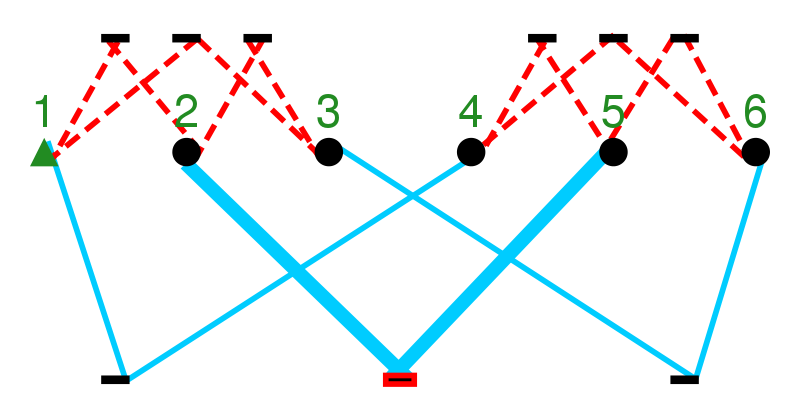
\includegraphics[width=0.7\textwidth]{h2_base.png}}
		\caption{bj-phi representation of a PHP instance of size 2}
		\label{fig:h2-graph}
	\end{centering}
\end{figure}


The image represents the DIMACS-CNF file:

\begin{lstlisting}[label=h2-file, caption=PHP of size 2 DIMACS file,]
p cnf 6 9
-1 -2 0
-1 -3 0
-2 -3 0

-4 -5 0
-4 -6 0
-5 -6 0

1 4 0
2 5 0
3 6 0
\end{lstlisting}

Where dashed lines represent negative literals and solid lines represent positive literals. Circles represent variables and little rectangles represent clauses.

In Figure \ref{fig:h2-graph} the thick little rectangle joining two thick solid lines  represent the clause [2 5 0] of line 11 in Listing \ref{h2-file}.

The graphs shown in the HTML page have more implicit information:

\begin{figure}[H]
	\begin{centering}
		\frame{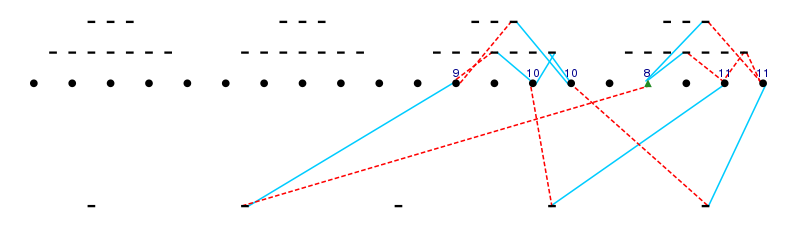
\includegraphics[width=0.9\textwidth]{h4_find1.png}}
		\caption{bj-phi graph for the first time PHP-2 is matched within PHP-4 solving}
		\label{fig:h4-f1}
	\end{centering}
\end{figure}

The equivalent consecutive numbering of variables shown in Figure \ref{fig:h2-graph} is assumed in Figure \ref{fig:h4-f1} according to their position from left to right, therefore the numbering shown in Figure \ref{fig:h4-f1} is not that of the literal but the ''tier'' of the ''charged'' {\quanton}. In Figure \ref{fig:h4-f1} variable 17 was charged in tier 8, variable 12 has tier 9, variables 14 and 15 have tier 10, and variables 19 and 20 have tier 11.

The dashed and solid lines in Figure \ref{fig:h4-f1} do not represent the sign of literals as in Figure \ref{fig:h2-graph}. In Figure \ref{fig:h4-f1} the signs of literals are also assumed according to their position in the graph: all above the circles are negative and all below are positive. 

The dashed lines and solid lines in Figure \ref{fig:h4-f1} represent the current assignation of a variable: 

\begin{enumerate}
\item
If the lines match the original state (were dashed and still dashed) the variable is positively charged.

\item
If they do not match the original, the variable is negatively charged.
\end{enumerate}

In Figure \ref{fig:h4-f1} variables 12, 19 and 20 are positive, and variables 14, 15 and 17 are negative.

The little triangle indicates a choice therefore in Figure \ref{fig:h4-f1} variable 17 is a choice.

\subsection{Results}
\label{subsect:results}

The following graph show the great difference between CDCL solvers and trainable solvers like ben-jose when solving PHP instances.

\begin{figure}[H]
	\begin{centering}
		\frame{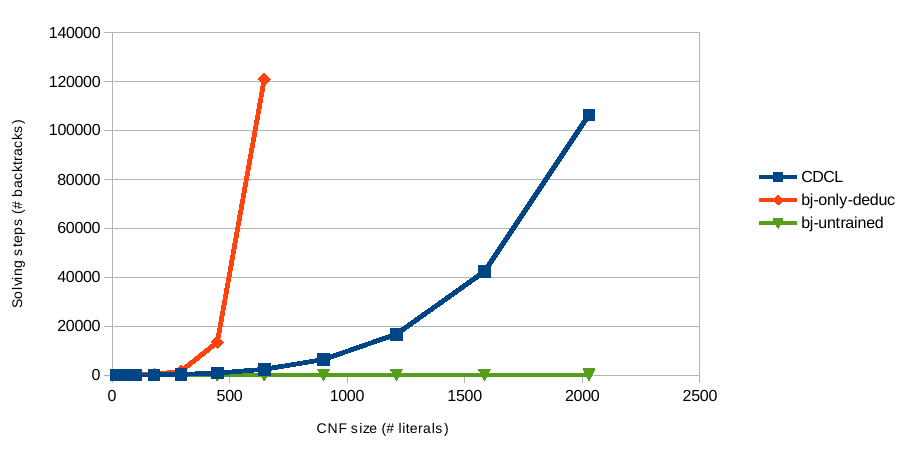
\includegraphics[width=0.7\textwidth]{results_01.png}}
		\caption{PHP SAT solving}
		\label{fig:results-1}
	\end{centering}
\end{figure}

The size of the CNF corresponds to the number of literals of CNFs for PHP-2, PHP-3, PHP-4, etc. 

The number of backtracks corresponds to number of laps (LAPS) in the output of \texttt{bj-batch-solver}

The only-deduc results were obtained with commands like:

\begin{verbatim}
	cd ben-jose-master/src/programs/tests/pigeon/
	bj-batch-solver h02.cnf -only_deduc
	bj-batch-solver h03.cnf -only_deduc
	bj-batch-solver h04.cnf -only_deduc
	...
\end{verbatim}

The only deduct has the same big \texttt{O} complexity than CDCL but is slower mainly to the modifications needed in ben-jose to be trainable (see Section \ref{sect:comparison}).

For the output of CDCL use your favorite solver.

The untrained (clean before each run) results were obtained with commands like:

\begin{verbatim}
	cd ben-jose-master/src/programs/tests/pigeon/
	sh clean_sh
	bj-batch-solver h02.cnf
	sh clean_sh
	bj-batch-solver h03.cnf
	sh clean_sh
	bj-batch-solver h04.cnf
	...
\end{verbatim}


The following graph show the big difference between trained and untrained solving with ben-jose when solving PHP instances.

\begin{figure}[H]
	\begin{centering}
		\frame{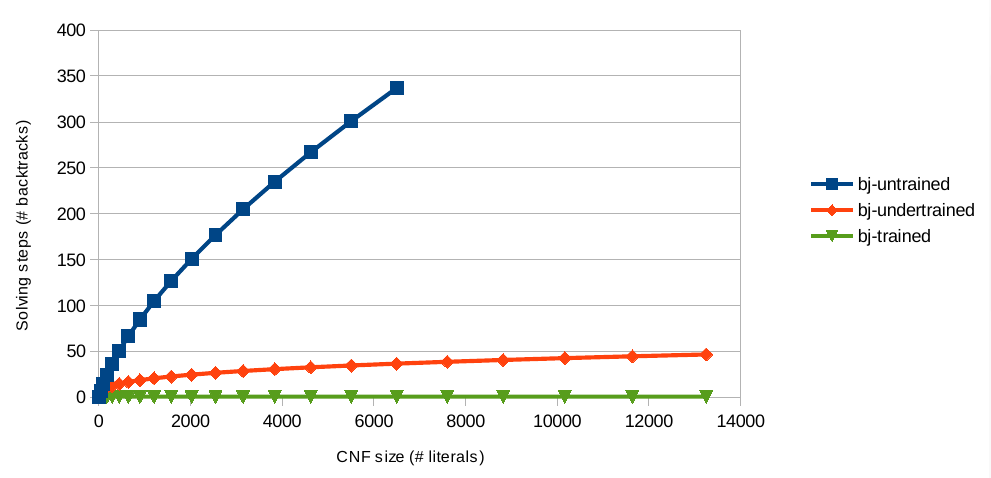
\includegraphics[width=0.7\textwidth]{results_02.png}}
		\caption{BJ PHP SAT solving}
		\label{fig:results-2}
	\end{centering}
\end{figure}



The under-trained (clean once) results were obtained with commands like:

\begin{verbatim}
	cd ben-jose-master/src/programs/tests/pigeon/
	sh clean_sh
	bj-batch-solver h02.cnf
	bj-batch-solver h03.cnf
	bj-batch-solver h04.cnf
	...
\end{verbatim}

The trained results (do not clean) were obtained repeating the under-trained commands without cleaning (deleting SKELETON).


%------------------------------------------------------------------------------
\section{Installation}
\label{sect:installation}

To install ben-jose:

\begin{enumerate}
\item
Download and unzip a ZIP file from the library from \url{https://github.com/joseluisquiroga/ben-jose}.

\item
\begin{verbatim}
	cd ben-jose-master/build/gnu_make
\end{verbatim}

\item
\begin{verbatim}
	make -s
\end{verbatim}

\item
\begin{verbatim}
	cd lib/ben-jose
\end{verbatim}

\item
\begin{verbatim}
	ls
\end{verbatim}
\end{enumerate}

That will built and list all the files of the library. Put the directory in the path.

%------------------------------------------------------------------------------
\subsection{Required Packages}

There are minimal requirements for building and compiling ben-jose:

\begin{itemize}
\item
A Linux system.

\item
GNU c++ (g++) installed.

\item
GMP Library (gmpxx) installed.
\end{itemize}

Almost every Linux system comes with the second two in the basic installation, so there is basically one requirement: a Linux system.

%------------------------------------------------------------------------------
\section{Comparison with other tools}
\label{sect:comparison}

\subsection{Trainable}

The most important difference of ben-jose with any other solver available today is the fact that it matches sub-formulas to already known to be unsatisfiable formulas (BCFFs) in order to skip the search on sub-formulas that match.

That technique allows this solver to be trainable. It holds a database of BCFFs that can be reused in later instances of SAT.

In order to archive this behavior some important modifications had to be done to the standard way of doing DPLL+BCP+CDCL. Learned clauses ({\neuron}s) are kept only until they are backtracked. That imposes a performance penalty when that clause can actually prune the search after it has been backtracked since it has to be deduced again by RES.

\subsection{Monos}

They are variables ({\quanton}s) that occur either only in positive form, or only in negative form after a BCP step, that is a level has been processed ({\leveldat} hold the data for levels). In the code they are called ''monos''. So:

\begin{itemize}
\item
When it is detected that there are only positons of a variable in the current sub-formula, the variable can safely be assumed to be set ''true''. 

\item
When it is detected that there are only negatons of a variable in the current sub-formula, the variable can safely be assumed to be set ''false''. 
\end{itemize}

This difference is crucial for to ease the matching of BCFFs.

\subsection{Longest BCP}

The solver uses a kind of ''look up technique'' that always chooses the ''longest'' path for BCP. 

When ever a choice is been made it tries both values in order to see which value propagates more variables. 

This difference is also crucial for to ease the matching of BCFFs.

In the code it can bee seen in the function ''start\_propagation'' when it calls ''select\_propag\_side''.

%------------------------------------------------------------------------------
\section{Future Work}
\label{sect:future-work}

Things to do with ben-jose:

\begin{itemize}
\item
Reduce combinatoric redundancy for dirty PHP instances (PHP with added redundant or side-effect clauses).

\item
Automate testing. Then: test, test and test. And when necessary: debug, debug and debug.

\item
Make an alpha release.

\item
Write more documentation for the software.

\item
Finish \texttt{-proof} option.

\item
Follow in detail for is-prime instances. It implies writing code to generate cytoscape.js graphs that help visualize the solving process.

\item
Simplify code that comes from research stages and works but now can be simpler.

\item
Write a concurrent version of ben-jose. Since a search branch can use the work done by an other search branch (use BCFFs written by the other branch) it is conceptually efficient to do concurrency.

The code has already considered this possibility by using the file system as a database and considering concurrency during file access.

\end{itemize}


%------------------------------------------------------------------------------
\section{Acknowledgments}
\label{sect:acknowledgments}

\begin{enumerate}
\item
Our heavenly Father YHWH (Yahweh).

\item
Our Lord Yashua (Jesus Christ).

\item
Magda Beltran de Quiroga (my mother).

\item
Federman Quiroga Rios (my father).

\item
Joao Marquez da Silva for his work on the SAT problem.

\item
All the authors in the bibliography.

\end{enumerate}

%------------------------------------------------------------------------------
\label{sect:bib}
\bibliographystyle{plain}
\bibliography{ben-jose}

%------------------------------------------------------------------------------
\end{document}

